\chapter{Base de dados orientada a grafos - Neo4J}
\paragraph{}
Além da migração para uma base de dados não relacional orientada a documentos, também implementamos um modelo na base de dados \textbf{Neo4j}, conhecida por sua orientação a grafos. Após uma análise aprofundada do nosso esquema relacional inicial, identificamos as relações mais significativas que podem ser representadas de forma eficiente neste paradigma não relacional.

O Neo4j permite a modelagem de dados em termos de nós e relacionamentos, proporcionando uma representação intuitiva das interconexões entre os dados. Com base nessa abordagem, identificamos e selecionamos os nós mais relevantes para representar corretamente as informações no Neo4j. Além disso, escolhemos as relações mais significativas para o nosso esquema relacional, traduzindo-as para estruturas de grafos que preservam a integridade das relações existentes. 
O schema da nossa base de dados ficou da seguinte forma:
\begin{figure}[h!]
    \centering
    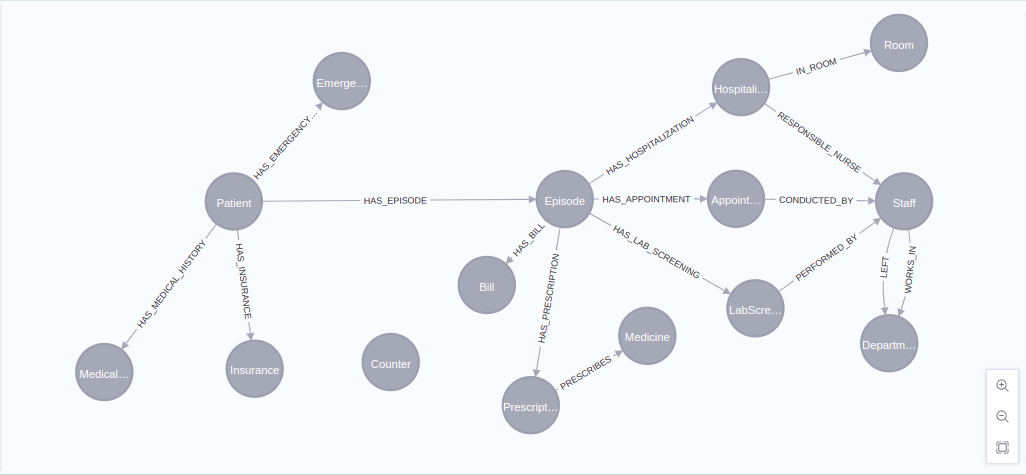
\includegraphics[width=0.95\linewidth]{Imagens/Neo4j/esquema_neo4j.png}
    \caption{Esquema da nossa base de dados Neo4j}
    \label{fig:esquema_neo4js}
\end{figure}

O esquema final no Neo4j inclui várias entidades (nós) e suas inter-relações, modelando de forma precisa o contexto hospitalar. A nossa estruturação de dados final têsm os 15 nós seguintes:

\begin{enumerate}
    \item \texttt{Paciente (Patient)}: Este nó representa todos os pacientes que já tiveram algum episódio hospitalar, exibindo os campos originais presentes na base de dados SQL. \ref{secPaciente}
    \item \texttt{Seguro de Saúde (Insurance)}: Este nó é representativo de vários seguros de saúde e contém os mesmos campos encontrados na tabela correspondente na base de dados SQL. \ref{secSeguroSaude}
    \item \texttt{Histórico Médico (Medical History)}: Este nó contém o histórico médico detalhado de cada paciente, mantendo os campos originais presentes na tabela SQL correspondente. \ref{secHistoricoMedico}
    \item \texttt{Contactos de Emergência (Emergency Contacts)}: Este nó representa os contactos de emergência dos pacientes, com os mesmos campos encontrados na tabela SQL correspondente. \ref{secContactosEmergencia}
    \item \texttt{Episódios Médicos (Episodes)}: Este nó é responsável por registar todos os episódios médicos de cada paciente, mantendo os campos originais da tabela correspondente presentes na base de dados SQL. \ref{secEpisodiosMedicos}
    \item \texttt{Faturas (Bill)}: Este nó representa as faturas associadas aos serviços prestados aos pacientes, mantendo os mesmos campos da tabela SQL correspondente. \ref{secFaturas}
    \item \texttt{Prescrição Médica (Prescription)}: Este nó contém informações sobre as prescrições médicas emitidas aos pacientes, mantendo a estrutura da tabela correspondente em SQL. \ref{secPrescricaoMedica}
    \item Medicamento (Medicine): Este nó representa os medicamentos disponíveis no hospital, mantendo os mesmos campos da tabela SQL correspondente. \ref{secMedicamento}
    \item \texttt{Departamento (Department)}: Este nó representa os diferentes departamentos do hospital, mantendo os parâmetros da tabela correspondente em SQL.\ref{secDepartamento}
    \item \texttt{Funcionários (Staff)}: Este nó reúne todas as tabelas referentes aos funcionários do nosso hospital, incluindo médicos, enfermeiros e técnicos. Dado que as estruturas das tabelas SQL para esses três tipos de funcionários são muito semelhantes, decidimos adotar uma abordagem semelhante ao MongoDB, abstraindo estas três tabelas e reunindo todos os elementos em um único nó denominado \texttt{staff}. Neste nó, apenas adicionamos um campo \texttt{role}, responsável por determinar a função do funcionário (DOCTOR, NURSE, TECHNICIAN). Para os funcionários com o papel de médico (\texttt{DOCTOR}), também adicionamos um campo \texttt{qualification}, característico da tabela \texttt{doctor} no SQL. \ref{secFuncionarios}
    \item \texttt{Consulta (Appointment):} Este nó regista as consultas marcadas pelos pacientes, mantendo os campos originais presentes na base de dados SQL. \ref{secConsulta}
    \item \texttt{Testes Médicos (Lab Screenings)}: Este nó contém informações sobre os testes médicos realizados nos pacientes, mantendo os mesmos campos da tabela SQL correspondente. \ref{secTestesMedicos}
    \item \texttt{Hospitalização (Hospitalization)}: Este nó regista informações sobre a hospitalização dos pacientes, mantendo os campos originais presentes na base de dados SQL. \ref{secHospitalizacao}
    \item \texttt{Quarto (Room)}: Este nó representa os quartos presentes no hospital. Os parâmetros deste nó são os mesmos da tabela correspondente na base de dados SQL.\ref{secQuarto}
    \item \texttt{Contador (Counter)}: Este nó auxiliar serve como um contador de IDs para os vários tipos de nós que possuem identificadores. Utilizando este nó, é possível obter um ID único sempre que um dos restantes tipos de nós seja adicionado, mantendo, desta forma, a integridade dos dados na base de dados Neo4j.\ref{secContador}
\end{enumerate}

No esquema final temos 16 relações entre os nós anteriormente mencionados. As relações são as seguintes:

\begin{enumerate}
    \item \texttt{HAS\_APPOINTMENT}: Representa a relação entre um paciente (\textit{patient}) e uma consulta agendada (\textit{appointment}). Um nó de paciente possui essa relação com um nó de consulta, indicando que o paciente tem uma consulta marcada.
    \item  \texttt{HAS\_BILL}: Reflete a relação entre um episódio médico (\textit{episode}) e uma fatura associada (\textit{bill}) a esse episódio. Um nó de episódio médico está conectado a um nó de fatura, indicando que ao episódio encontra-se associada uma fatura.
    \item  \texttt{HAS\_EMERGENCY\_CONTACT}: Indica a relação entre um paciente (\textit{patient}) e um contato de emergência (\textit{emergency contact}). Um nó de paciente está conectado a um ou mais nós de contato de emergência, representando que o paciente possui um ou mais contatos de emergência registados.
    \item  \texttt{HAS\_EPISODE}: Reflete a relação entre um paciente (\textit{patient}) e um episódio médico (\textit{episode}). Um nó de paciente possui essa relação com um nó de episódio médico, indicando que o paciente está envolvido nesse episódio e correlacionando assim o paciente com os elementos médicos.
    \item  \texttt{HAS\_HOSPITALIZATION}: Representa a relação entre um episódio médico (\textit{episode}) e uma hospitalização (\textit{hospitalization}) associada a esse episódio. Um nó de episódio médico está conectado a um nó de hospitalização, indicando que o episódio médico recorreu a uma hospitalização do paciente a qual o episódio se encontra associado.
    \item  \texttt{HAS\_INSURANCE}: Indica a relação entre um paciente (\textit{patient}) e um seguro de saúde (\textit{insurance}). Um nó de paciente possui essa relação com um nó de seguro de saúde, indicando qual o seguro de saúde do paciente em questão.
    \item  \texttt{HAS\_MEDICAL\_HISTORY}: Reflete a relação entre um paciente (\textit{patient}) e seu histórico médico (\textit{medical history}). Um nó de paciente está conectado a um ou mais nós de histórico médico, indicando que o paciente tem um ou mais nós de histórico médico registados.
    \item  \texttt{HAS\_PRESCRIPTION}: Denota a relação entre um episódio médico (\textit{episode}) e uma prescrição (\textit{prescription}) associada a esse episódio. Um nó de episódio médico está conectado a um ou mais nós de prescrição, indicando que o episódio possui uma ou mais prescrições.
    \item  \texttt{IN\_ROOM}: Representa a relação entre uma hospitalização (\textit{hospitalization}) e o quarto (\textit{room}) onde o paciente está internado. Um nó de hospitalização está conectado a um nó de quarto, indicando o quarto onde a hospitalização ocorre. Um nó de quarto pode ter associado várias hospitalizações desde que em horários que não coincidam.
    \item  \texttt{LEFT}: Indica a relação entre um paciente (\textit{patient}) e sua hospitalização (\textit{hospitalization}), semelhante ao que ocorre com a relação HAAS\_HOSPITALIZATION, no entanto, neste caso apenas os pacientes que já abandonaram uma hospitalização apresentam esta relação, ou seja, pacientes com alta hospitalar. Um nó de paciente possui essa relação com um nó de hospitalização, representando que o paciente teve alta do hospital.
    \item  \texttt{PRESCRIBES}: Reflete a relação entre um médico (\textit{doctor}) e uma prescrição (\textit{prescription}) que ele emite. Um nó de médico está conectado a um ou mais nós de prescrição, indicando que o médico emitiu a prescrição.
    \item  \texttt{RESPONSIBLE\_NURSE}: Indica a relação entre uma hospitalização (\textit{hospitalization}) e a enfermeira responsável (\textit{nurse}) por essa hospitalização. Um nó de hospitalização está conectado a um nó de enfermeira, representando que a enfermeira é responsável por essa hospitalização.
    \item  \texttt{CONDUCTED\_BY}: Representa a relação entre uma consulta agendada (\textit{appointment}) e o médico que a realizou. Um nó de consulta está conectado a um nó de médico, indicando que o médico conduziu a consulta.
    \item  \texttt{WORKS\_IN}: Denota a relação entre um funcionário (médico, enfermeiro, técnico) e o departamento (\textit{department}) em que ele trabalha. Um nó de funcionário possui essa relação com um nó de departamento, indicando que o funcionário trabalha no departamento.
    \item  \texttt{HAS\_LAB\_SCREENING}: Representa a relação entre um episódio médico (\textit{episode}) e um exame laboratorial (\textit{lab screening}) associado a esse episódio. Um nó de episódio médico está conectado a um ou mais nós de exame laboratorial, indicando que o episódio médico incluiu a realização de um ou mais exames exame.
    \item  \texttt{PERFORMED\_BY}: Reflete a relação entre um exame laboratorial (\textit{lab screening}) e um técnico (\textit{technician}) responsável por realizá-lo. Um nó de exame laboratorial está conectado a um nó de técnico, indicando que o técnico foi o responsável pela execução do exame laboratorial. O mesmo técnico pode ser responsável pela realização de vários exames laboratoriais.
\end{enumerate}

\section{\textit{Constraints} em Neo4j}

A migração de dados de Oracle para Neo4j envolveu a definição de várias \textit{constraints} para assegurar a integridade e a unicidade dos dados na base de dados orientada a grafos. As \textit{constraints} adicionadas garantem que os dados inseridos no Neo4j respeitam a unicidade dos ids, quando os mesmos existem, prevenindo duplicações e mantendo a consistência das informações armazenadas. A seguir, detalhamos as 14 \textit{constraints} implementadas:
\begin{enumerate}
    \item Pacientes (\textit{Patient}): Para garantir que cada paciente é único na base de dados, foi criada uma \textit{constraint} para assegurar a unicidade do identificador de paciente (\texttt{id\_patient}), assim, adicionamos uma \textit{constraint} ao identificador deste nó garantindo que não existem dois pacientes com o mesmo ID. 

    \begin{myminted}{cypher}
    CREATE CONSTRAINT FOR (p:Patient) REQUIRE p.id_patient IS UNIQUE
    \end{myminted}

    \item Seguros de Saúde (\textit{Insurance}): De modo a evitar duplicações nas apólices de seguro, foi adicionada uma constraint de unicidade para o número da apólice (policy\_number). 

    \begin{myminted}{cypher}
    CREATE CONSTRAINT FOR (i:Insurance) REQUIRE i.policy_number IS UNIQUE
    \end{myminted}
    
    \item Contatos de Emergência (\textit{Emergency Contact}): Para garantir que para este tipo de nó cada combinação de nome de contato, telefone e relação é única, foi criada uma \textit{constraint} composta incluindo estes três parâmetros.
    
    \begin{myminted}{cypher}
    CREATE CONSTRAINT unique_contact FOR (c:EmergencyContact) REQUIRE (c.contact_name, c.phone, c.relation) IS UNIQUE
    \end{myminted}
    
    \item Histórico Médico (\textit{Medical History}): Cada registo de histórico médico (\texttt{id\_record}) deve ser único para assegurar a integridade dos dados históricos dos pacientes, adicionamos, assim, uma \textit{constraint} no identificador deste nó como forma de garantir que não existem dois registos de histórico médico iguais.

    \begin{myminted}{cypher}
    CREATE CONSTRAINT FOR (m:MedicalHistory) REQUIRE m.id_record IS UNIQUE
    \end{myminted}
    
    \item Departamentos (\textit{Department}): Os departamentos são identificados de forma única pelo seu identificador de departamento (\texttt{id\_department}), ao colocarmos uma \textit{constraint} única no seu identificador garantimos que não é possível existir dois departamentos com o mesmo ID.
    
    \begin{myminted}{cypher}
    CREATE CONSTRAINT FOR (dep:Department) REQUIRE dep.id_department IS UNIQUE
    \end{myminted}

    \item Funcionários (\textit{Staff}): Para assegurar a unicidade dos funcionários na base de dados, foi adicionada uma \textit{constraint} no identificador do funcionário (\texttt{id\_emp}), desta forma garantimos que não existem dois funcionários com o mesmo ID.

    \begin{myminted}{cypher}
    CREATE CONSTRAINT FOR (s:Staff) REQUIRE s.id_emp IS UNIQUE
    \end{myminted}
    
    \item Quartos (\textit{Room}): Cada quarto ligado à hospitalização é identificado de forma única pelo seu identificador de quarto (\texttt{id\_room}), pelo que, apenas é necessário incluir uma \textit{constraint} neste identificador, garantindo que não existam dois quartos com o mesmo ID.

    \begin{myminted}{cypher}
    CREATE CONSTRAINT FOR (r:Room) REQUIRE r.id_room IS UNIQUE
    \end{myminted}
    
    \item Faturas (\textit{Bill}): As faturas são únicas e identificadas pelo seu identificador de fatura (\texttt{id\_bill}), assim sendo, apenas é necessário incluir uma \textit{constraint} neste identificador, garantindo que não existam duas faturas com o mesmo ID.
    
    \begin{myminted}{cypher}
    CREATE CONSTRAINT FOR (b:Bill) REQUIRE b.id_bill IS UNIQUE
    \end{myminted}
    
    \item Medicamentos (\textit{Medicine}): Cada medicamento é identificado de forma única pelo seu identificador de medicamento (\texttt{id\_medicine}), pelo que, apenas é necessário incluir uma \textit{constraint} neste identificador, garantindo que não existam dois medicamentos com o mesmo ID.
    
    \begin{myminted}{cypher}
    CREATE CONSTRAINT FOR (m:Medicine) REQUIRE m.id_medicine IS UNIQUE
    \end{myminted}
    
    \item Prescrições (\textit{Prescription}): De modo a evitar a existência de duplicações nas prescrições, foi criada uma constraint no identificador da prescrição (\texttt{id\_prescription}), garantindo que não existem duas prescrições com o mesmo ID.
    
    \begin{myminted}{cypher}
    CREATE CONSTRAINT FOR (p:Prescription) REQUIRE p.id_prescription IS UNIQUE  
    \end{myminted}
    
    \item Exames Laboratoriais (\textit{Lab Screening}): Cada exame laboratorial é identificado de forma única pelo seu identificador de exame (\texttt{id\_lab}), pelo que, apenas é necessário incluir uma \textit{constraint} neste identificador, garantindo que não existam dois exames laboratoriais com o mesmo ID.
    
    \begin{myminted}{cypher}
    CREATE CONSTRAINT FOR (l:LabScreening) REQUIRE l.id_lab IS UNIQUE
    \end{myminted}
    
    \item Consultas (\textit{Appointment}): Sendo que o nó não apresenta um identificador único, foi utilizado uma \textit{constraint} composta para garantir que as consultas são únicas. Uma consulta é identificadas pela combinação da data, hora e identificador do médico responsável, garantindo que um mesmo médico não pode dar duas consultas numa mesma data e hora. 
    
    \begin{myminted}{cypher}
    CREATE CONSTRAINT unique_appointment FOR (a:Appointment) REQUIRE(a.appointment_date, a.appointment_time, a.id_doctor) IS UNIQUE
    \end{myminted}
    
    \item Hospitalizações (\textit{Hospitalization}): Uma vez que este nó não apresenta um identificador único e para assegurar a unicidade das hospitalizações, foi criada uma \textit{constraint} composta que considera a data de admissão e o identificador do episódio médico, garantindo que duas hospitalizações na mesma data têm de ser feitas por episódios médicos diferentes, ou seja, para pacientes diferentes. 
    
    \begin{myminted}{cypher}
    CREATE CONSTRAINT unique_hospitalization FOR (h:Hospitalization) REQUIRE (h.admission_date, h.id_episode) IS UNIQUE
    \end{myminted}
    
    \item Episódios Médicos (\textit{Episode}): Cada episódio médico é identificado de forma única pelo seu identificador de episódio (\texttt{id\_episode}), pelo que apenas é necessário incluir uma \textit{constraint} neste identificador, garantindo que não existam dois episódios com o mesmo ID.
    
    \begin{myminted}{cypher}
    CREATE CONSTRAINT FOR (e:Episode) REQUIRE e.id_episode IS UNIQUE
    \end{myminted}
\end{enumerate}

\section{Triggers em Neo4j}

Durante o processo de migração de dados da base de dados Oracle para Neo4j, foi necessário definir diversos \textit{triggers} para otimizar a inserção de novos nós e manter a integridade dos dados. Na nossa base de dados, procurávamos evitar o uso manual de campos de identificação durante a inserção de novos nós. Para isso, utilizamos \textit{triggers} que gerassem automaticamente esses identificadores, garantindo a integridade e a unicidade dos dados.

Para alcançar este objetivo, introduzimos um nó auxiliar (\textit{Counter}) que armazena o número máximo dos identificadores utilizados até o momento. Este nó facilita a geração de novos identificadores únicos para futuros nós. Assim, após a inserção de um novo nó, os \textit{triggers} eram acionados para obter o próximo identificador a partir do nó \textit{Counter}, incrementar o contador presente neste nó, de acordo com o seu tipo, e atribuir o novo identificador ao nó recém-criado.

Além dos \textit{triggers} relacionados à criação de identificadores únicos, foi necessário adaptar um \textit{trigger} existente na base de dados original Oracle para o ambiente Neo4j. Este \textit{trigger} específico foi ajustado para garantir que sua funcionalidade fosse preservada após a migração, mantendo a consistência e a continuidade das operações automatizadas.

Em Neo4j, para a correta criação dos triggers, foi necessário recorrer à biblioteca \textbf{APOC} (\textit{Awesome Procedures on Cypher}). A biblioteca APOC fornece acesso a procedimentos e funções definidos pelos utilizadores que estendem o uso da linguagem de consulta \textit{Cypher} para novas áreas. Utilizando os recursos avançados oferecidos pela APOC, conseguimos automatizar e otimizar a criação e gestão de identificadores únicos para novos nós.

\subsection{Triggers para a adição de identificadores únicos}

Na sequencia da criação destes \textit{triggers} foi observado a existência de algumas consistências entre o nome do nó (\texttt{label}) e o nome do ID (\texttt{id\_ + label}). Estas consistências dividiram a implementação em dois tipos principais: \textit{triggers} dinâmicos para \textit{labels} comuns e \textit{triggers} específicos para \textit{labels} com nomes de identificador diferentes do nome da \textit{label}.

Os dados de transações em Neo4j são transformados em estruturas de dados apropriadas para serem consumidas como parâmetros nas instruções. Recorremos, portanto, à variável \texttt{\$createdNodes} que permite, quando um nó é criado no Neo4j, acionar o nosso \textit{trigger}. O parâmetro \texttt{\$createdNodes} é uma lista que contém os nós recém-criados durante a transação. Esta lista é então utilizada pelos \textit{triggers} para executar operações específicas, como, no nosso caso, a criação de identificadores únicos.

Assim sendo, para as \textit{labels}: \textit{Patient}, \textit{Room}, \textit{Department}, \textit{Episode}, \textit{Medicine}, \textit{Prescription} e \textit{Bill}, foi criado um único \textit{trigger} que fosse acionados com a inserção de nós das \textit{labels} mencionadas.

\begin{myminted}{cypher}
CALL apoc.trigger.install(
    'hospital',
    'dynamic_id_trigger',
    '
    UNWIND |\$|createdNodes AS n
    WITH n, head(apoc.node.labels(n)) AS label
    WITH n, label, \'id_\' + toLower(label) AS dynamicProperty
    WITH n, label, apoc.map.get(n, dynamicProperty, false) as idValue, dynamicProperty
    MATCH (c:Counter {type: label})
    WHERE label in ["Patient","Room","Department","Episode","Medicine","Prescription","Bill"] AND NOT idValue 
    CALL apoc.cypher.run("
        MATCH (c:Counter {type: |\$|label})
        RETURN c.count + 1 AS count
    ", {label: label}) YIELD value
    CALL apoc.create.setProperty(n, dynamicProperty, value.count) YIELD node
    SET n = node
    SET c.count = value.count
    ',
    {phase: 'afterAsync'}
);
\end{myminted}

Como podemos observar o procedimento seguido foi o seguinte:
\begin{enumerate}
    \item Instalar o \textit{trigger} denominado \texttt{dynamic\_id\_trigger} na base de dados \textbf{hospital}.
    \item Descompactar os nós criados (\textit{unwind}).
    \item Obter a \textit{label} que sofreu uma transação.
    \item Verifica se o nó não possui a propriedade do identificador (\texttt{apoc.map.get(n, dynamicProperty, false)}).
    \item Verifica se o nó é um dos nós onde existe uma consistência entre a \textit{label} e o nome do ID, só estes nós é que serão alterados com este \textit{trigger}.
    \item Incrementa o contador correspondente à \textit{label} e atribui o valor ao novo nó.
\end{enumerate}

Para os restantes \textit{triggers}, o processo é semelhante, a única diferença reside na forma como são identificados os nós e atribuídos os identificadores únicos. Cada \textit{trigger} é configurado para operar em um tipo específico de nó, verificando se esse nó já possui um identificador associado. Se não, é gerado um novo identificador único com base no contador (\textit{Counter}) correspondente ao tipo de nó. Esse identificador é então atribuído ao nó antes de atualizar o contador para refletir a adição do novo nó na base de dados. Assim, todos os \textit{triggers} garantem que os nós criados recebam identificadores únicos de forma automática e consistente, mantendo a integridade dos dados na base de dados Neo4j.

\subsection{Trigger proveniente da base de dados Oracle}

O \textit{trigger} proveniente da base de dados Oracle em questão têm como objetivo principal gerar automaticamente uma fatura (\textit{Bill}) quando um paciente recebe uma alta hospitalar, ou seja, quando ao nó hospitalização (\textit{hospitalization}), que é responsável por manter a informação sobre a hospitalização do paciente, é acrescentado o campo referente à data da alta hospitalar (\texttt{discharge\_date}). 

No ambiente Oracle, este \textit{trigger} era implementado para monitorizar a inserção do campo de alta hospitalar e, ao detetar essa inserção, iniciava uma série de processos para calcular os custos associados ao paciente durante sua estadia. Esses custos incluíam taxas de quarto (\texttt{room\_cost}), custos de exames laboratoriais (\texttt{test\_cost}) e outros encargos médicos (\texttt{other\_charges}). A soma total desses custos resultava na criação de uma nova fatura, que então era vinculada ao episódio de hospitalização do paciente.

Para a criação deste \textit{trigger} foi necessário recorrer à propriedade \texttt{\$assignedNodeProperties} da biblioteca \textit{apoc.trigger} para monitorizar mudanças nos nós. Esta propriedade é um mapa que contém chaves para listas de mapas, onde cada mapa inclui a chave \textit{(key)}, o valor antigo (\textit{old}), o valor novo (\textit{new}) e o nó (\textit{node}). O \textit{trigger} é ativado quando a propriedade \texttt{discharge\_date} é atribuída a um nó \textit{Hospitalization}.

O trigger obtido em Neo4j foi o seguinte:
\begin{myminted}{cypher}
    CALL apoc.trigger.install(
    'hospital',
    'trg_generate_bill',
    '
    UNWIND keys(\$assignedNodeProperties) AS k
    WITH k
    WHERE k = \'discharge_date\'
    UNWIND |\$|assignedNodeProperties[k] AS map
    WITH map.node AS h, map.old AS old, map.new AS new
    WHERE "Hospitalization" IN LABELS(h) AND old IS NULL AND new IS NOT NULL
    MATCH (e:Episode)-[:HAS_HOSPITALIZATION]->(h)
    MATCH (h)-[:IN_ROOM]->(r:Room)
    WITH e, h, COALESCE(r.room_cost, 0) AS v_room_cost
    OPTIONAL MATCH (e)-[:HAS_LAB_SCREENING]->(ls:LabScreening)
    WITH e, h, v_room_cost, COALESCE(SUM(ls.test_cost), 0) AS v_test_cost
    OPTIONAL MATCH (e)-[:HAS_PRESCRIPTION]->(p:Prescription)-[:PRESCRIBES]->(m:Medicine)
    WITH e, h, v_room_cost, v_test_cost, COALESCE(SUM(m.m_cost * p.dosage), 0) AS v_other_charges
    WITH e, v_room_cost, v_test_cost, v_other_charges, (v_room_cost + v_test_cost + v_other_charges) AS v_total_cost
    MATCH (c:Counter {type: \'Bill\'})
   CALL apoc.cypher.run("
        MATCH (c:Counter {type: \'Bill\'})
        RETURN c.count + 1 AS count
    ",{}) YIELD value
     CREATE (b:Bill {
        id_bill: value.count,
        room_cost: v_room_cost,
        test_cost: v_test_cost,
        other_charges: v_other_charges,
        total: v_total_cost,
        id_episode: e.id_episode,
        registered_at: datetime(),
        payment_status: "PENDING"
    })
    MERGE (e)-[:HAS_BILL]->(b)
    SET c.count = value.count
',
    {phase: 'afterAsync'}
);
\end{myminted}

O procedimento levado a cabo pelo \textit{trigger} apresentado acima é o seguinte:
\begin{enumerate}
    \item Instalação do \textit{trigger}.
    \item  Monitorização da Propriedade do nó de hospitalização, de forma a percecionar quando uum nó de hospitalização é atualizado com a inserção do campo \textit{discharge\_date} .
    \item  Cálculo de Custos associados com a hospitalização, recolhendo os custos do quarto associado à hospitalização (\texttt{\_room\_cost}), possíveis custos referentes à realização de testes laboratoriais (\texttt{v\_test\_cost}), e ainda possíveis despesas com a prescrição de medicação (\texttt{v\_other\_charges}). No final realizando o custo total da hospitalização, que estará presente na fatura, através da soma dos vários valores anteriormente referidos.
    \item  Criação de uma fatura (nó \textit{Bill}), recorrendo às variáveis, \texttt{v\_room\_cost}, \texttt{v\_test\_cost} e \texttt{v\_other\_charges}.
    \item  Associação da fatura ao episódio correspondente à hospitalização.
\end{enumerate}

Este trigger garante que a transição do OracleDB para o Neo4j mantenha a mesma eficiência e precisão na criação de faturas, assegurando a continuidade das operações financeiras no ambiente hospitalar de uma forma otimizada.

\section{Exploração da Base de Dados}

Após a migração para o Neo4J, conforme explicado anteriormente, iniciámos a exploração desta base de dados orientada a grafos. Para isso, utilizamos \textbf{queries} ou \textbf{expressões} tanto para passar um ID de uma tabela específica e obter a informação desejada, bem como, passar mais do que um parâmetro para obter dados de forma mais precisa e que englobassem mais do que um nó.

Por exemplo, para obter todas as informações de um paciente específico, incluindo detalhes sobre seus episódios médicos, consultas agendadas, faturas, hospitalizações e exames laboratoriais, utilizamos uma \textit{query} que recebe como parâmetro o \textit{id\_patient}. A \textit{query} percorre todos os nós que possuem estas informações apenas para o ID passado como parâmetro, fazendo uso das ligações entre eles para poder obter informação sobre cada um dos campos acima mencionados. Abaixo encontra-se a implementação desta \textit{query}:

\begin{myminted}{javascript}
MATCH (p:Patient {id_patient: 89})
OPTIONAL MATCH (p)-[:HAS_EPISODE]->(e:Episode)
OPTIONAL MATCH (e)-[:HAS_APPOINTMENT]->(appointment:Appointment)
OPTIONAL MATCH (e)-[:HAS_BILL]->(bill:Bill)
OPTIONAL MATCH (e)-[:HAS_HOSPITALIZATION]->(hospitalization:Hospitalization)
OPTIONAL MATCH (e)-[:HAS_LAB_SCREENING]->(lab:LabScreening)
RETURN p, 
       COLLECT(DISTINCT appointment) AS appointments, 
       COLLECT(DISTINCT bill) AS bills, 
       COLLECT(DISTINCT hospitalization) AS hospitalizations, 
       COLLECT(DISTINCT lab) AS labScreenings
\end{myminted}

Analisando a \textit{query} de forma concreta, temos:

\begin{myminted}{javascript}
MATCH (p:Patient {id_patient: 89})
\end{myminted}

Encontra o nó Patient com a campo \textit{id\_patient} igual a 89.

\begin{myminted}{javascript}
OPTIONAL MATCH (p)-[:HAS_EPISODE]->(e:Episode)
\end{myminted}

Realiza um \textit{match} opcional (que pode ou não existir) para encontrar todos os episódios médicos (\textit{Episode}) associados ao paciente. A relação \textit{HAS\_EPISODE} conecta o paciente aos seus episódios médicos.

\begin{myminted}{javascript}
OPTIONAL MATCH (e)-[:HAS_APPOINTMENT]->(appointment:Appointment)
\end{myminted}

Realiza um \textit{match} opcional para encontrar todas as consultas (\textit{Appointment}) associadas aos episódios médicos do paciente. A relação \textit{HAS\_APPOINTMENT} conecta os episódios médicos às suas consultas.

\begin{myminted}{javascript}
OPTIONAL MATCH (e)-[:HAS_BILL]->(bill:Bill)
\end{myminted}

Realiza um \textit{match} opcional para encontrar todas as faturas (\textit{Bill}) associadas aos episódios médicos do paciente. A relação \textit{HAS\_BILL} conecta os episódios médicos às suas faturas.

\begin{myminted}{javascript}
OPTIONAL MATCH (e)-[:HAS_HOSPITALIZATION]->(hospitalization:Hospitalization)
\end{myminted}

Realiza um \textit{match} opcional para encontrar todas as hospitalizações (\textit{Hospitalization}) associadas aos episódios médicos do paciente. A relação \textit{HAS\_HOSPITALIZATION} conecta os episódios médicos às suas hospitalizações.

\begin{myminted}{javascript}
OPTIONAL MATCH (e)-[:HAS_LAB_SCREENING]->(lab:LabScreening)
\end{myminted}

Realiza um \textit{match} opcional para encontrar todos os exames laboratoriais (\textit{LabScreening}) associados aos episódios médicos do paciente. A relação \textit{HAS\_LAB\_SCREENING} conecta os episódios médicos aos seus exames laboratoriais.

É importante mencionar que a utilização de uma base de dados orientada a grafos, como o Neo4j, oferece várias vantagens para o bom desempenho da \textit{query} fornecida. Vantagens como a \textbf{Consulta Rápida de Relacionamentos} que envolvem a navegação através de relações entre entidades, faz com que esta \textit{query} que envolve múltiplos relacionamentos (paciente para episódios, episódios para consultas, faturas, hospitalizações e exames), seja executada de forma muito eficiente. Outra vantagem que é importante mencionar é a \textbf{Travessia de Grafo} onde o Neo4J utiliza técnicas de travessia de grafo que permitem encontrar e retornar dados relacionados de forma rápida, mesmo com grandes volumes de dados.

\subsection{Operações Básicas em Neo4J}

Numa base de dados NoSQL como o Neo4J, não é necessário implementar funções separadas para realizar operações básicas como inserir, apagar ou atualizar nós. O Neo4J fornece métodos internos para lidar diretamente com estas operações. Aqui está um breve resumo de como pode realizar estas operações no Neo4J:

\begin{itemize}
    \item \textbf{Inserir Nós e Relacionamentos:} Para inserir um nó ou um relacionamento, pode usar-se o comando \texttt{CREATE}.
    \item \textbf{Apagar Nós e Relacionamentos:} Para apagar nós ou relacionamentos, pode usar-se o comando \texttt{DELETE}.
    \item \textbf{Atualizar Nós e Relacionamentos:} Para atualizar propriedades de nós ou relacionamentos, pode usar o comando \texttt{SET}. Para remover propriedades, pode usar o comando \texttt{REMOVE}.
\end{itemize}

O Neo4J, sendo uma base de dados NoSQL, é projetado para manipular dados de forma mais flexível e direta, eliminando a necessidade de mecanismos de controlo adicionais nas operações de \textbf{Criação} (\textit{CREATE}), \textbf{Atualização} (\textit{UPDATE}) e \textbf{Remoção} (\textit{DELETE}). 

\subsection{Visão Paciente}

\vspace{0.15cm} 
\textbf{Buscar todos os pacientes:} Esta query retorna todos os pacientes registados na base de dados. Cada paciente é representado por um nó \texttt{Patient}.

\vspace{0.15cm} 
\textbf{Buscar paciente por ID:} Retorna o nó \texttt{Patient} que tem um ID específico. Utiliza a propriedade \texttt{id\_patient} para encontrar o paciente desejado.

\vspace{0.15cm} 
\textbf{Buscar historial médico para um dado ID:} Retorna o nó \texttt{Patient} e todos os nós \texttt{MedicalHistory} relacionados a ele através da relação \texttt{HAS\_MEDICAL\_HISTORY}. Cada nó \texttt{MedicalHistory} contém informações sobre condições médicas passadas do paciente.

\vspace{0.15cm} 
\textbf{Buscar seguro para um dado ID:} Retorna os detalhes do seguro do paciente específico. Encontra o nó \texttt{Patient} com o ID fornecido e segue a relação \texttt{HAS\_INSURANCE} para obter o nó \texttt{Insurance} associado.

\vspace{0.15cm} 
\textbf{Buscar contacto de emergência para um dado ID:} Retorna os detalhes do contacto de emergência do paciente específico. Encontra o nó \texttt{Patient} com o ID fornecido e segue a relação \texttt{HAS\_EMERGENCY\_CONTACT} para obter o nó \texttt{EmergencyContact} associado.

\vspace{0.15cm} 
\textbf{Buscar pacientes por tipo de sangue:} Retorna todos os pacientes com um tipo de sangue específico. Utiliza a propriedade \texttt{blood\_type} do nó \texttt{Patient} para encontrar todos os pacientes com o tipo sanguíneo fornecido.

\vspace{0.15cm} 
\textbf{Buscar pacientes por género:} Retorna todos os pacientes de um género específico (masculino ou feminino). Utiliza a propriedade \texttt{gender} do nó \texttt{Patient} para filtrar os pacientes pelo género.

\vspace{0.15cm} 
\textbf{Buscar pacientes pela condição médica:} Retorna todos os pacientes que têm uma condição médica específica. Encontra todos os nós \texttt{Patient} que têm uma relação \texttt{HAS\_MEDICAL\_HISTORY} com um nó \texttt{MedicalHistory} onde a condição corresponde à fornecida.

\vspace{0.15cm} 
\textbf{Buscar todos os tipos de relações em contactos de emergência:} Retorna todos os tipos de relações registadas nos nós \texttt{EmergencyContact}. Cada relação descreve a natureza do contacto de emergência com o paciente (por exemplo, pai, mãe).

\vspace{0.15cm} 
\textbf{Buscar todos os tipos de provedores de seguro:} Retorna todos os provedores de seguro disponíveis na base de dados. Cada provedor é identificado pela propriedade \texttt{provider}.

\vspace{0.15cm} 
\textbf{Buscar todos os tipos de planos de seguro:} Retorna todos os diferentes planos de seguro registados nos nós \texttt{Insurance}. Cada plano é identificado pela propriedade \texttt{insurance\_plan}.

\vspace{0.15cm} 
\textbf{Buscar todos os tipos de cobertura:} Retorna todos os diferentes tipos de cobertura registados nos nós \texttt{Insurance}. Cada tipo de cobertura é identificado pela propriedade \texttt{coverage}.

\vspace{0.15cm} 
\textbf{Buscar historial médico:} Retorna todos os registros de historial médico na base de dados. Cada registro é representado por um nó \texttt{MedicalHistory}.

\vspace{0.15cm} 
\textbf{Buscar seguro:} Retorna todos os registros de seguro na base de dados. Cada registro é representado por um nó \texttt{Insurance}.

\vspace{0.15cm}
\textbf{Buscar contacto de emergência:} Retorna todos os registros de contactos de emergência na base de dados. Cada registro é representado por um nó \texttt{EmergencyContact}.

\vspace{0.15cm} 
\textbf{Buscar todos os tipos de condições médicas:} Retorna todos os diferentes tipos de condições médicas registadas nos nós \texttt{MedicalHistory}. Cada condição é identificada pela propriedade \texttt{condition}.

\vspace{0.15cm} 
\textbf{Buscar todos os tipos sanguíneos:} Retorna todos os diferentes tipos sanguíneos registados nos nós \texttt{Patient}. Cada tipo sanguíneo é identificado pela propriedade \texttt{blood\_type}.

\vspace{0.15cm} 
\textbf{Buscar número de pacientes para cada tipo sanguíneo:} Retorna o número de pacientes para cada tipo sanguíneo, ordenado pela quantidade de pacientes. Conta quantos nós \texttt{Patient} existem para cada valor de \texttt{blood\_type}.

\vspace{0.15cm} 
\textbf{Buscar número de pacientes para cada condição médica:} Retorna o número de pacientes para cada condição médica, ordenado pela quantidade de pacientes. Conta quantos nós \texttt{Patient} têm uma relação \texttt{HAS\_MEDICAL\_HISTORY} com um nó \texttt{MedicalHistory} para cada valor de \texttt{condition}.

\vspace{0.15cm} 
\textbf{Buscar pacientes por provedor de seguro específico:} Retorna todos os pacientes que têm seguro com um provedor específico. Encontra os nós \texttt{Patient} que têm uma relação \texttt{HAS\_INSURANCE} com um nó \texttt{Insurance} onde o provedor corresponde ao fornecido.

\vspace{0.15cm} 
\textbf{Buscar pacientes por plano de seguro específico:} Retorna todos os pacientes que têm um plano de seguro específico. Encontra os nós \texttt{Patient} que têm uma relação \texttt{HAS\_INSURANCE} com um nó \texttt{Insurance} onde o plano corresponde ao fornecido.

\vspace{0.15cm} 
\textbf{Buscar pacientes por cobertura específica:} Retorna todos os pacientes que têm uma cobertura de seguro específica. Encontra os nós \texttt{Patient} que têm uma relação \texttt{HAS\_INSURANCE} com um nó \texttt{Insurance} onde a cobertura corresponde à fornecida.

\vspace{0.15cm} 
\textbf{Buscar pacientes dentro de um intervalo de idades:} Retorna todos os pacientes nascidos entre datas específicas. Utiliza a propriedade \texttt{birthday} do nó \texttt{Patient} para filtrar os pacientes dentro do intervalo de datas fornecido.

\vspace{0.15cm}
\textbf{Buscar pacientes com cobertura de maternidade:} Retorna todos os pacientes que têm cobertura de maternidade no seguro. Encontra os nós \texttt{Patient} que têm uma relação \texttt{HAS\_INSURANCE} com um nó \texttt{Insurance} onde a cobertura de maternidade é verdadeira.

\vspace{0.15cm} 
\textbf{Buscar pacientes com cobertura dental:} Retorna todos os pacientes que têm cobertura dental no seguro. Encontra os nós \texttt{Patient} que têm uma relação \texttt{HAS\_INSURANCE} com um nó \texttt{Insurance} onde a cobertura dental é verdadeira.

\vspace{0.15cm} 
\textbf{Buscar pacientes com cobertura óptica:} Retorna todos os pacientes que têm cobertura óptica no seguro. Encontra os nós \texttt{Patient} que têm uma relação \texttt{HAS\_INSURANCE} com um nó \texttt{Insurance} onde a cobertura óptica é verdadeira.

\vspace{0.15cm} 
\textbf{Buscar pacientes com várias combinações de cobertura:} Retorna pacientes que têm várias combinações de coberturas (por exemplo, dental e óptica). Encontra os nós \texttt{Patient} que têm uma relação \texttt{HAS\_INSURANCE} com um nó \texttt{Insurance} onde múltiplas coberturas são verdadeiras.

\vspace{0.15cm} 
\textbf{Buscar pacientes por relação de contacto de emergência:} Retorna todos os pacientes cujo contacto de emergência tem uma relação específica (por exemplo, pai). Encontra os nós \texttt{Patient} que têm uma relação \texttt{HAS\_EMERGENCY\_CONTACT} com um nó \texttt{EmergencyContact} onde a relação corresponde à fornecida.

\vspace{0.15cm} 
\textbf{Buscar paciente pelo primeiro e último nome:} Retorna o paciente com um primeiro e último nome específico. Utiliza as propriedades \texttt{patient\_fname} e \texttt{patient\_lname} do nó \texttt{Patient} para encontrar o paciente.

\vspace{0.15cm} 
\textbf{Buscar paciente pelo número de telefone:} Retorna o paciente com um número de telefone específico. Utiliza a propriedade \texttt{phone} do nó \texttt{Patient} para encontrar o paciente.

\vspace{0.15cm} 
\textbf{Contar o número de pacientes:} Retorna a contagem total de pacientes registados na base de dados. Conta todos os nós \texttt{Patient}.

\vspace{0.15cm} 
\textbf{Buscar pacientes com um contacto de emergência específico:} Retorna todos os pacientes cujo contacto de emergência é uma pessoa específica. Encontra os nós \texttt{Patient} que têm uma relação \texttt{HAS\_EMERGENCY\_CONTACT} com um nó \texttt{EmergencyContact} onde o nome do contacto corresponde ao fornecido.

\vspace{0.15cm} 
\textbf{Buscar pacientes pelo ID do historial médico:} Retorna todos os pacientes que têm um historial médico com um ID específico. Encontra os nós \texttt{Patient} que têm uma relação \texttt{HAS\_MEDICAL\_HISTORY} com um nó \texttt{MedicalHistory} onde o ID do historial corresponde ao fornecido.

\subsection{Visão Staff}

\vspace{0.15cm}
\textbf{Buscar toda a Informação de um Staff:} Retorna todas as informações do funcionário cujo ID é fornecido. Utiliza a propriedade \texttt{id\_emp} para encontrar o funcionário desejado.

\vspace{0.15cm}
\textbf{Buscar o Department para um dado ID:} Retorna o funcionário com um ID específico e o departamento em que ele trabalha. Também pode buscar diretamente um departamento pelo seu ID.

\vspace{0.15cm}
\textbf{Buscar toda a informação das Enfermeiras:} Retorna todas as informações de todos os funcionários cujo papel é \textit{NURSE}. Utiliza a propriedade \texttt{role} para filtrar os funcionários.

\vspace{0.15cm}
\textbf{Buscar toda a informação dos Médicos:} Retorna todas as informações de todos os funcionários cujo papel é \textit{DOCTOR}. Utiliza a propriedade \texttt{role} para filtrar os funcionários.

\vspace{0.15cm}
\textbf{Buscar toda a informação dos Técnicos:} Retorna todas as informações de todos os funcionários cujo papel é \textit{TECHNICIAN}. Utiliza a propriedade \texttt{role} para filtrar os funcionários.

\vspace{0.15cm}
\textbf{Buscar quantos Enfermeiros existem:} Retorna a contagem de todos os funcionários cujo papel é \textit{NURSE}. Utiliza a propriedade \texttt{role} para contar os funcionários.

\vspace{0.15cm}
\textbf{Buscar quantos Doutores existem:} Retorna a contagem de todos os funcionários cujo papel é \textit{DOCTOR}. Utiliza a propriedade \texttt{role} para contar os funcionários.

\vspace{0.15cm}
\textbf{Buscar quantos Técnicos existem:} Retorna a contagem de todos os funcionários cujo papel é \textit{TECHNICIAN}. Utiliza a propriedade \texttt{role} para contar os funcionários.

\vspace{0.15cm}
\textbf{Buscar quantos enfermeiros, doutores e técnicos existem:} Retorna a contagem de funcionários agrupados por seus papéis (\textit{NURSE}, \textit{DOCTOR}, \textit{TECHNICIAN}). Utiliza a propriedade \texttt{role} para agrupar e contar os funcionários.

\vspace{0.15cm}
\textbf{Buscar quantos Departamentos existem:} Retorna a contagem de todos os departamentos na base de dados. Conta todos os nós \texttt{Department}.

\vspace{0.15cm}
\textbf{Buscar Staff por Data de Admissão:} Retorna todos os funcionários que foram admitidos na data fornecida. Utiliza a propriedade \texttt{date\_joining} para filtrar os funcionários.

\vspace{0.15cm}
\textbf{Buscar Staff por Data de Separação:} Retorna todos os funcionários que se separaram na data fornecida. Utiliza a propriedade \texttt{date\_separation} para filtrar os funcionários.

\vspace{0.15cm}
\textbf{Buscar Staff Ativo ou Inativo:} Retorna todos os funcionários que estão ativos ou inativos. Utiliza a propriedade \texttt{is\_active\_status} para filtrar os funcionários.

\vspace{0.15cm}
\textbf{Qualificações de um Doctor por ID:} Retorna as qualificações do doutor cujo ID é fornecido. Utiliza as propriedades \texttt{role} e \texttt{id\_emp} para encontrar o doutor.

\vspace{0.15cm}
\textbf{Todos os tipos de Qualificações:} Retorna todas as qualificações distintas dos doutores. Utiliza a propriedade \texttt{qualification} para listar as qualificações únicas.

\vspace{0.15cm}
\textbf{Número de Empregados por Departamento:} Retorna a contagem de funcionários por departamento. Utiliza a relação \texttt{WORKS\_IN} para agrupar e contar os funcionários por departamento.

\vspace{0.15cm}
\textbf{Enfermeiros por Departamento:} Retorna a contagem de enfermeiros por departamento. Utiliza a propriedade \texttt{role} e a relação \texttt{WORKS\_IN} para agrupar e contar os enfermeiros por departamento.

\vspace{0.15cm}
\textbf{Número de Doutores por Departamento:} Retorna a contagem de doutores por departamento. Utiliza a propriedade \texttt{role} e a relação \texttt{WORKS\_IN} para agrupar e contar os doutores por departamento.

\vspace{0.15cm}
\textbf{Número de Técnicos por Departamento:} Retorna a contagem de técnicos por departamento. Utiliza a propriedade \texttt{role} e a relação \texttt{WORKS\_IN} para agrupar e contar os técnicos por departamento.

\vspace{0.15cm}
\textbf{Contar Quantos Staff Estão Ativos:} Retorna a contagem de todos os funcionários que estão ativos. Utiliza a propriedade \texttt{is\_active\_status} para contar os funcionários ativos.

\vspace{0.15cm}
\textbf{Contar Quantos Staff não estão Ativos:} Retorna a contagem de todos os funcionários que não estão ativos. Utiliza a propriedade \texttt{is\_active\_status} para contar os funcionários inativos.

\vspace{0.15cm}
\textbf{Buscar Staff pelo Primeiro Nome e Sobrenome:} Retorna o funcionário cujo primeiro nome e sobrenome correspondem aos fornecidos. Utiliza as propriedades \texttt{emp\_fname} e \texttt{emp\_lname} para encontrar o funcionário.

\vspace{0.15cm}
\textbf{Buscar Staff pelo Email:} Retorna o funcionário cujo email corresponde ao fornecido. Utiliza a propriedade \texttt{email} para encontrar o funcionário.

\vspace{0.15cm}
\textbf{Contar o Número Total de Staff:} Retorna a contagem total de funcionários registados na base de dados. Conta todos os nós \texttt{Staff}.

\vspace{0.15cm}
\textbf{Buscar Staff pelo SSN:} Retorna o funcionário cujo número de segurança social (SSN) corresponde ao fornecido. Utiliza a propriedade \texttt{ssn} para encontrar o funcionário.

\subsection{Visão Episodes}

\vspace{0.15cm}
\textbf{Buscar toda a informação de um Episódio por ID:} Retorna todas as informações do episódio cujo ID é fornecido. Utiliza a propriedade \texttt{id\_episode} para encontrar o episódio desejado.

\vspace{0.15cm}
\textbf{Buscar toda a informação sobre Prescrições Hospitalares:} Retorna todas as informações de todas as prescrições registadas na base de dados.

\vspace{0.15cm}
\textbf{Quantos episódios para um dado paciente:} Retorna a contagem de episódios associados a um paciente específico. Utiliza a relação \texttt{HAS\_EPISODE} para contar os episódios de um paciente.

\vspace{0.15cm}
\textbf{Buscar as prescrições para um dado ID de episódio:} Retorna todas as prescrições associadas a um episódio específico. Utiliza a relação \texttt{HAS\_PRESCRIPTION} para obter as prescrições de um episódio.

\vspace{0.15cm}
\textbf{Buscar bill para um dado ID de episódio:} Retorna todas as contas associadas a um episódio específico. Utiliza a relação \texttt{HAS\_BILL} para obter as contas de um episódio.

\vspace{0.15cm}
\textbf{Buscar bill por ID de conta:} Retorna a conta cujo ID é fornecido. Utiliza a propriedade \texttt{id\_bill} para encontrar a conta desejada.

\vspace{0.15cm}
\textbf{Buscar exames laboratoriais para um dado ID de episódio:} Retorna todos os exames laboratoriais associados a um episódio específico. Utiliza a relação \texttt{HAS\_LAB\_SCREENING} para obter os exames de um episódio.

\vspace{0.15cm}
\textbf{Buscar exame laboratorial por ID de laboratório:} Retorna o exame laboratorial cujo ID é fornecido. Utiliza a propriedade \texttt{id\_lab} para encontrar o exame desejado.

\vspace{0.15cm}
\textbf{Buscar hospitalização para um dado ID de episódio:} Retorna todas as hospitalizações associadas a um episódio específico. Utiliza a relação \texttt{HAS\_HOSPITALIZATION} para obter as hospitalizações de um episódio.

\vspace{0.15cm}
\textbf{Buscar sala por ID de sala:} Retorna a sala cujo ID é fornecido. Utiliza a propriedade \texttt{id\_room} para encontrar a sala desejada.

\vspace{0.15cm}
\textbf{Buscar prescrições por ID de paciente:} Retorna todas as prescrições associadas a um paciente específico. Utiliza a propriedade \texttt{patient\_id} e a relação \texttt{HAS\_PRESCRIPTION} para obter as prescrições do paciente.

\vspace{0.15cm}
\textbf{Buscar bills por ID de paciente:} Retorna todas as contas associadas a um paciente específico. Utiliza a propriedade \texttt{patient\_id} e a relação \texttt{HAS\_BILL} para obter as contas do paciente.

\vspace{0.15cm}
\textbf{Buscar exames laboratoriais por ID de paciente:} Retorna todos os exames laboratoriais associados a um paciente específico. Utiliza a propriedade \texttt{patient\_id} e a relação \texttt{HAS\_LAB\_SCREENING} para obter os exames do paciente.

\vspace{0.15cm}
\textbf{Buscar hospitalização por ID de paciente:} Retorna todas as hospitalizações associadas a um paciente específico. Utiliza a propriedade \texttt{patient\_id} e a relação \texttt{HAS\_HOSPITALIZATION} para obter as hospitalizações do paciente.

\vspace{0.15cm}
\textbf{Buscar sala por ID de paciente:} Retorna todas as salas associadas a um paciente específico. Utiliza a propriedade \texttt{patient\_id}, a relação \texttt{HAS\_HOSPITALIZATION}, e a relação \texttt{IN\_ROOM} para obter as salas do paciente.

\vspace{0.15cm}
\textbf{Buscar medicamento por ID de paciente:} Retorna todos os medicamentos associados a um paciente específico. Utiliza a propriedade \texttt{patient\_id}, a relação \texttt{HAS\_PRESCRIPTION}, e a relação \texttt{PRESCRIBES} para obter os medicamentos do paciente.

\vspace{0.15cm}
\textbf{Buscar prescrições por ID de paciente e data:} Retorna todas as prescrições associadas a um paciente específico e uma data específica. Utiliza a propriedade \texttt{patient\_id}, a relação \texttt{HAS\_PRESCRIPTION}, e a propriedade \texttt{prescription\_date} para filtrar as prescrições.

\vspace{0.15cm}
\textbf{Buscar hospitalizações por ID de paciente e data de admissão:} Retorna todas as hospitalizações associadas a um paciente específico e uma data de admissão específica. Utiliza a propriedade \texttt{patient\_id}, a relação \texttt{HAS\_HOSPITALIZATION}, e a propriedade \texttt{admission\_date} para filtrar as hospitalizações.

\vspace{0.15cm}
\textbf{Buscar todas as prescrições de um paciente específico:} Retorna todas as prescrições de um paciente específico, independentemente do episódio. Utiliza a propriedade \texttt{patient\_id} e a relação \texttt{HAS\_PRESCRIPTION}.

\vspace{0.15cm}
\textbf{Buscar todas as contas de um paciente específico:} Retorna todas as contas de um paciente específico, independentemente do episódio. Utiliza a propriedade \texttt{patient\_id} e a relação \texttt{HAS\_BILL}.

\vspace{0.15cm}
\textbf{Buscar todos os exames laboratoriais de um paciente específico:} Retorna todos os exames laboratoriais de um paciente específico, independentemente do episódio. Utiliza a propriedade \texttt{patient\_id} e a relação \texttt{HAS\_LAB\_SCREENING}.

\vspace{0.15cm}
\textbf{Buscar todas as hospitalizações de um paciente específico:} Retorna todas as hospitalizações de um paciente específico, independentemente do episódio. Utiliza a propriedade \texttt{patient\_id} e a relação \texttt{HAS\_HOSPITALIZATION}.

\vspace{0.15cm}
\textbf{Buscar todas as salas de um paciente específico:} Retorna todas as salas de um paciente específico, independentemente do episódio. Utiliza a propriedade \texttt{patient\_id}, a relação \texttt{HAS\_HOSPITALIZATION}, e a relação \texttt{IN\_ROOM}.

\vspace{0.15cm}
\textbf{Buscar todas as informações de um episódio específico:} Retorna todas as informações detalhadas de um episódio específico, incluindo prescrições, contas, hospitalizações e exames laboratoriais. Utiliza a propriedade \texttt{id\_episode} para encontrar o episódio e suas relações associadas.

\vspace{0.15cm}
\textbf{Buscar todas as informações de todos os episódios:} Retorna todas as informações detalhadas de todos os episódios, incluindo prescrições, contas, hospitalizações e exames laboratoriais. Utiliza as relações associadas aos episódios.

\vspace{0.15cm}
\textbf{Buscar informações do médico responsável por um episódio específico:} Retorna todas as informações do médico responsável por um episódio específico. Utiliza a relação \texttt{HAS\_APPOINTMENT} e a relação \texttt{CONDUCTED\_BY} para obter o médico.

\vspace{0.15cm}
\textbf{Buscar todas as informações dos médicos que atenderam um paciente específico:} Retorna todas as informações dos médicos que atenderam um paciente específico. Utiliza a relação \texttt{HAS\_EPISODE}, a relação \texttt{HAS\_APPOINTMENT}, e a relação \texttt{CONDUCTED\_BY} para obter os médicos.

\vspace{0.15cm}
\textbf{Buscar informações do técnico responsável por um episódio específico:} Retorna todas as informações do técnico responsável por um episódio específico. Utiliza a relação \texttt{HAS\_LAB\_SCREENING} e a relação \texttt{PERFORMED\_BY} para obter o técnico.

\vspace{0.15cm}
\textbf{Buscar todas as informações dos técnicos que atenderam um paciente específico:} Retorna todas as informações dos técnicos que atenderam um paciente específico. Utiliza a relação \texttt{HAS\_EPISODE}, a relação \texttt{HAS\_LAB\_SCREENING}, e a relação \texttt{PERFORMED\_BY} para obter os técnicos.

\vspace{0.15cm}
\textbf{Retornar informações de um paciente específico dado um ID de paciente:} Retorna todas as informações de um paciente específico, incluindo todos os episódios, consultas, contas, hospitalizações e exames laboratoriais. Utiliza a propriedade \texttt{id\_patient} e as relações associadas.

\vspace{0.15cm}
\textbf{Retornar informações de todos os pacientes:} Retorna todas as informações detalhadas de todos os pacientes, incluindo todos os episódios, consultas, contas, hospitalizações e exames laboratoriais. Utiliza as relações associadas aos pacientes.

\subsection{Visão Global}

\vspace{0.15cm}
\textbf{Listar todas as prescrições para um paciente específico:} Retorna todas as prescrições associadas a um paciente específico. Utiliza a relação \texttt{HAS\_EPISODE} para encontrar os episódios do paciente e a relação \texttt{HAS\_PRESCRIPTION} para obter as prescrições desses episódios.

\vspace{0.15cm}
\textbf{Listar os pacientes alocados a um específico quarto:} Retorna todos os pacientes que estão alocados a um quarto específico. Utiliza a relação \texttt{IN\_ROOM} para encontrar as hospitalizações no quarto e a relação \texttt{HAS\_HOSPITALIZATION} para obter os episódios associados aos pacientes.

\vspace{0.15cm}
\textbf{Listar todos os internamentos de um determinado paciente:} Retorna todas as hospitalizações associadas a um paciente específico. Utiliza a relação \texttt{HAS\_EPISODE} para encontrar os episódios do paciente e a relação \texttt{HAS\_HOSPITALIZATION} para obter as hospitalizações desses episódios.

\vspace{0.15cm}
\textbf{Listar hospitalizações por enfermeira responsável:} Retorna todas as hospitalizações pelas quais uma enfermeira específica é responsável. Utiliza a relação \texttt{RESPONSIBLE\_NURSE} para encontrar as hospitalizações associadas ao enfermeiro.

\vspace{0.15cm}
\textbf{Listar todos os episódios médicos de um paciente específico:} Retorna todos os episódios médicos associados a um paciente específico. Utiliza a relação \texttt{HAS\_EPISODE} para encontrar os episódios do paciente.

\vspace{0.15cm}
\textbf{Listar episódios médicos por tipo de condição:} Retorna todos os episódios médicos associados a pacientes com uma condição médica específica. Utiliza a relação \texttt{HAS\_MEDICAL\_HISTORY} para encontrar os pacientes com a condição e a relação \texttt{HAS\_EPISODE} para obter os episódios desses pacientes.

\vspace{0.15cm}
\textbf{Listar todos os episódios médicos tratados por um médico específico:} Retorna todos os episódios médicos tratados por um médico específico. Utiliza a relação \texttt{CONDUCTED\_BY} para encontrar as consultas conduzidas pelo médico e a relação \texttt{HAS\_APPOINTMENT} para obter os episódios associados a essas consultas.

\vspace{0.15cm}
\textbf{Listar todos os exames laboratoriais para um paciente específico:} Retorna todos os exames laboratoriais associados a um paciente específico. Utiliza a relação \texttt{HAS\_EPISODE} para encontrar os episódios do paciente e a relação \texttt{HAS\_LAB\_SCREENING} para obter os exames desses episódios.

\vspace{0.15cm}
\textbf{Listar exames baseados no técnico responsável:} Retorna todos os exames laboratoriais realizados por um técnico específico. Utiliza a relação \texttt{PERFORMED\_BY} para encontrar os exames associados ao técnico.

\vspace{0.15cm}
\textbf{Listar todas as faturas para um paciente específico:} Retorna todas as faturas associadas a um paciente específico. Utiliza a relação \texttt{HAS\_EPISODE} para encontrar os episódios do paciente e a relação \texttt{HAS\_BILL} para obter as faturas desses episódios.

\vspace{0.15cm}
\textbf{Listar todas as consultas agendadas para um paciente específico:} Retorna todas as consultas agendadas associadas a um paciente específico. Utiliza a relação \texttt{HAS\_EPISODE} para encontrar os episódios do paciente e a relação \texttt{HAS\_APPOINTMENT} para obter as consultas desses episódios.

\vspace{0.15cm}
\textbf{Listar consultas baseadas no médico responsável:} Retorna todas as consultas conduzidas por um médico específico. Utiliza a relação \texttt{CONDUCTED\_BY} para encontrar as consultas associadas ao médico.

\vspace{0.15cm}
\textbf{Listar os Appointment para um dado Medico por dia:} Retorna todas as consultas agendadas para um médico específico em uma data específica. Utiliza a relação \texttt{CONDUCTED\_BY} e filtra pela data da consulta.

\vspace{0.15cm}
\textbf{Buscar Appointment por data:} Retorna todas as consultas agendadas em uma data específica. Utiliza a propriedade \texttt{appointment\_date} para filtrar as consultas.

\vspace{0.15cm}
\textbf{Buscar Appointment por data e depois por hora:} Retorna todas as consultas agendadas em uma data e hora específicas. Utiliza as propriedades \texttt{appointment\_date} e \texttt{appointment\_time} para filtrar as consultas.

\vspace{0.15cm}
\textbf{Lista todos os episódios e o respetivo paciente:} Retorna todos os episódios médicos e os pacientes associados. Utiliza a relação \texttt{HAS\_EPISODE} para obter os episódios e os pacientes correspondentes.

\vspace{0.15cm}
\textbf{Lista os médicos com mais consultas marcadas, com informação detalhada do paciente:} Retorna os médicos com mais consultas marcadas, incluindo informações detalhadas dos pacientes atendidos. Utiliza a relação \texttt{CONDUCTED\_BY} para encontrar as consultas, agrupa os médicos pelo número de consultas e coleta informações dos pacientes atendidos.
